
\begin{dialog}{无伴奏阿基里斯奏鸣曲}

\begin{quote}
电话响了,阿基里斯拿起话筒。
\end{quote}

\begin{dialogue}

\item[阿基里斯]喂,我是阿基里斯。

\item[阿基里斯]噢,你好,龟兄,你怎么样?

\item[阿基里斯]得了窝颈症?啊,真不幸。你自己知道是什么引起的吗?

\item[阿基里斯]你呆在那种姿态下有多久?

\item[阿基里斯]哦,难怪变得僵硬了。究竟是什么东西居然叫你那么长时间地拧着脖子?

\item[阿基里斯]其中有很多都挺怪模怪样的,是吗?都是些什么东西啊?举个例子?

\item[阿基里斯]你说什么——“魔幻般的各种动物”?

\begin{figure}
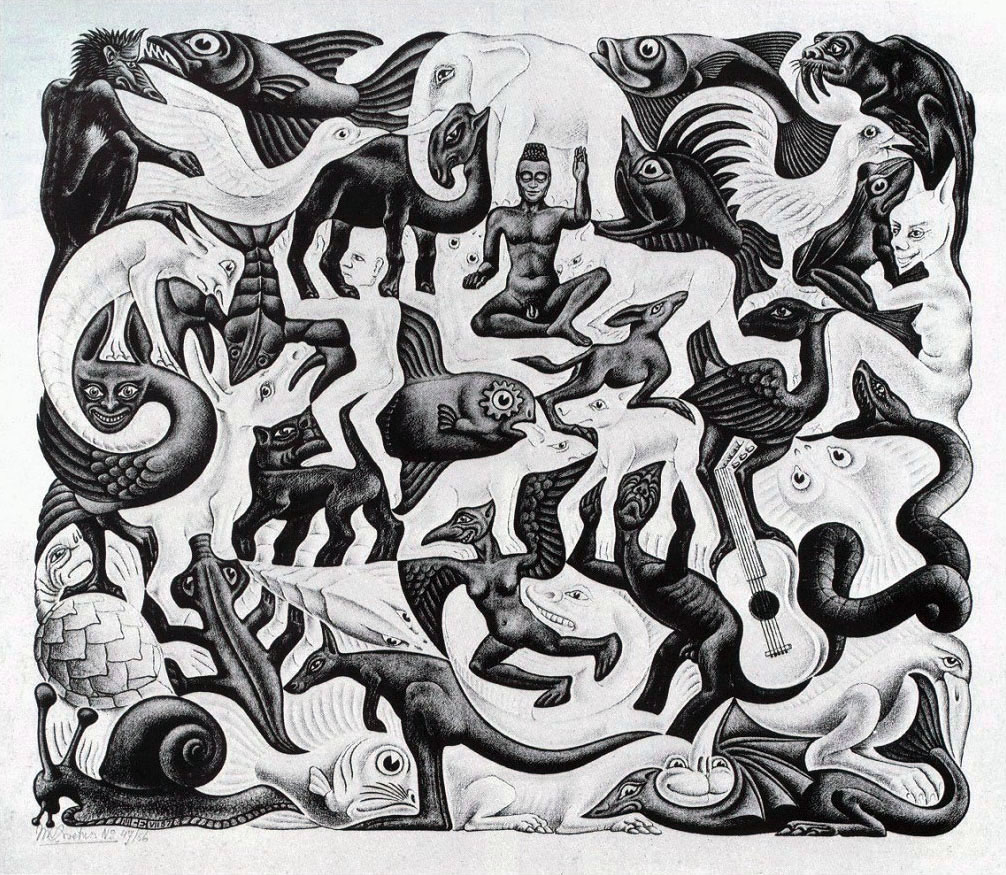
\includegraphics{img_014.jpg}
\caption[镶嵌画II,艾舍尔作。]
  {镶嵌画II,艾舍尔作(蚀版画,1957)。}
\end{figure}

\item[阿基里斯]你认出了你的朋友螃蟹?它干嘛要变成那种样子?什么?螃蟹总是爱把自己弄进最不可思议的困境里?这呆瓜!幸亏那对钳子没变样。

\item[阿基里斯]还有一把吉他?太奇怪啦。说到音乐,你想过来听一听那位最对你口味的作曲家巴赫的无伴奏小提琴奏鸣曲吗?我刚买到一张这些奏鸣曲的唱片,那效果真是太棒啦。我现在还没从那里面醒过劲儿来呢。巴赫只用了一把小提琴就创作出了这么有趣的作品!

\item[阿基里斯]怎么,还没劲儿?我知道到了你这样的岁数会怎么样。真遗憾,也许你应该上床读会儿书什么的。

\item[阿基里斯]哦,是吗,没电了?有时会出现这种情况的,不过我看你可以点上蜡烛。

\item[阿基里斯]哦,哦,原来是因为失眠,那最好就别看书了。可是,究竟是什么叫你睡不着觉呢?

\item[阿基里斯]哦,是这么回事啊。那好,如果是这个叫你一直神不守舍,那你也许最好说给我听听,让我和你一起来研究研究。

\item[阿基里斯]一个词,其居中的两个部首依次是“昔”和“火”……嗯……“秋鹊”怎么样?

\item[阿基里斯]的确,“昔”、“火”在这个词里顺序是颠倒的。

\item[阿基里斯]一连猜了几个小时?听起来我好像一头栽进了一个非常难解的字谜里了。这个该死的字谜你是打哪儿听来的?

\item[阿基里斯]你是说他看去像是在思索深奥的佛理,可实际上他只是在力图解开复杂的字谜,是吗?

\item[阿基里斯]啊哈!——原来是那只蜗牛知道这家伙在干什么。可是你怎么想起跟那只蜗牛说话的呢?

\item[阿基里斯]听我说,我曾经见过一个字谜,跟这个有点像。你想知道吗?这会不会弄得你更加神不守舍呢?

\item[阿基里斯]我也这么想——不会有任何害处的。下面就是那个字谜:什么词以部首“虫”开头,又以部首“虫”结尾?

\item[阿基里斯]真机灵——不过这近乎赖皮了。这当然不是我心里所想的那个答案。

\item[阿基里斯]你当然很对——它满足了条件,不过这是种“走捷径”的解决办法。我心里另有谜底。

\item[阿基里斯]叫你猜着了!你怎么这么快就想出来啦?

\item[阿基里斯]我明白了。事实上停电不仅没有耽误你的事,反而帮了你的忙。太妙了!可是对于你的那个“昔火”谜,我这儿还是一抹黑呢。

\item[阿基里斯]祝贺你!这样一来你也许能睡着了!告诉我吧,谜底是什么?

\item[阿基里斯]是的,我一般不喜欢提示,但是没关系,你要给我什么提示呢?

\item[阿基里斯]我不懂你在这里用“图形”和“衬底”是表示什么。

\item[阿基里斯]我当然知道《镶嵌画II》那幅画!我熟悉艾舍尔的所有作品。毕竟,他是我最喜欢的艺术家。我无论到哪儿总要在墙上挂一幅《镶嵌画II》的印刷复制品,我现在一抬眼就能看得见。

\item[阿基里斯]是的,我看出了所有的黑颜色动物。

\item[阿基里斯]对,我还看到它们中间的“负空间”——也就是剩下的画面——是些白颜色的动物图案。

\item[阿基里斯]你所说的“图形”和“衬底”原来是这个意思啊。可是这同那个“昔火”字谜有什么关系呢?

\item[阿基里斯]哦,对我来说这太复杂了。我真希望能马上来个“肚里点蜡烛——透心明白”。

\item[阿基里斯]没听说过?这可是我最喜欢的歇后语了。

\item[阿基里斯]你现在就准备过来?可是我刚才还想——

\item[阿基里斯]那好吧。也许到那时我会想出你那个字谜的正确答案,对,用你那个“图形—衬底”的暗示,把它同我的那个字谜联系起来。

\item[阿基里斯]我很愿意把它们放给你听。

\item[阿基里斯]你发明了一种有关它们的理论?

\item[阿基里斯]用什么乐器伴奏?

\item[阿基里斯]嗯,如果真是这样的话,他不愿写出羽管键琴部分并把它发表就有点奇怪了。

\item[阿基里斯]我懂了——带点儿随意的色彩。听它们可以有两种办法——带伴奏的或不带伴奏的。但是人们怎么会知道那伴奏听起来怎么样呢?

\item[阿基里斯]啊,对,我想那是最好的,把它留给听众去想象。况且还说不定正像你所说的那样,巴赫甚至从未想到过要有伴奏。这些奏鸣曲现在这样似乎也确实很好。

\item[阿基里斯]没错儿。好吧,一会儿见。

\item[阿基里斯]再见,龟兄。

\end{dialogue}

\end{dialog}
